%%%%%%%%%%%%%%%%%%%%%%%%%%%%%%%%%%%%%%%%%
% Research Report Assignment Title Page 
% LaTeX Template
% Version 1.0 (06/03/16)
%
% This template has been downloaded from:
% http://www.LaTeXTemplates.com
%
% Original author: Francisco Maria Calisto
% WikiBooks (http://en.wikibooks.org/wiki/LaTeX/Title_Creation)
%
% License:
% CC BY-NC-SA 3.0 (http://creativecommons.org/licenses/by-nc-sa/3.0/)
% 
% Instructions for using this template:
% This title page is capable of being compiled as is. This is not useful for 
% including it in another document. To do this, you have two options: 
%
% 1) Copy/paste everything between \begin{document} and \end{document} 
% starting at \begin{titlepage} and paste this into another LaTeX file where you 
% want your title page.
% OR
% 2) Remove everything outside the \begin{titlepage} and \end{titlepage} and 
% move this file to the same directory as the LaTeX file you wish to add it to. 
% Then add \input{./title_page_1.tex} to your LaTeX file where you want your
% title page.
%
%%%%%%%%%%%%%%%%%%%%%%%%%%%%%%%%%%%%%%%%%
%\title{Title page with logo}
%------------------------------------------------------------------------------
%	PACKAGES AND OTHER DOCUMENT CONFIGURATIONS
%------------------------------------------------------------------------------

\documentclass[12pt]{article}
\usepackage[english]{babel}
\usepackage[utf8x]{inputenc}
\usepackage[T1]{fontenc}
\usepackage{amsmath}
\usepackage{graphicx}
\usepackage[colorinlistoftodos]{todonotes}
\usepackage{subcaption}
\usepackage{biblatex}
\usepackage{fontspec}
\usepackage{pifont}

\addbibresource{bib.bib}

\begin{document}

\begin{titlepage}

\newcommand{\HRule}{\rule{\linewidth}{0.5mm}} % Defines a new command for the horizontal lines, change thickness here

\center % Center everything on the page
 
%------------------------------------------------------------------------------
%	HEADING SECTIONS
%------------------------------------------------------------------------------

% Name of your university/college
\textsc{\LARGE Instituto Superior T\'{e}cnico}\\[1.5cm]
% Major heading such as course name
\textsc{\Large ISR}\\[0.5cm]
% First Minor heading such as course title
\textsc{\large Report}\\[0.25cm]
% Second Minor heading such as course title
\textsc{\small Users and Tasks Analysis Milestone}\\[0.25cm]

%------------------------------------------------------------------------------
%	TITLE SECTION
%------------------------------------------------------------------------------

\HRule \\[0.5cm]
{ \large \bfseries Participatory User Tests Meeting \& Notes}\\[0.25cm] % Title of your document
\HRule \\[0.5cm]
 
%------------------------------------------------------------------------------
%	AUTHOR SECTION
%------------------------------------------------------------------------------

\begin{minipage}{0.4\textwidth}
\begin{flushleft} \large
\emph{Author:}\\
Francisco Maria \textsc{Calisto} % Your name
\end{flushleft}
\end{minipage}
~
\begin{minipage}{0.4\textwidth}
\begin{flushright} \large
\emph{Coordinator:} \\
Jacinto \textsc{Nascimento} % Coordinator's Name
\end{flushright}
~
\begin{flushright} \large
\emph{Co-Coordinator:} \\
Daniel \textsc{Gon\c{c}alves} % Co-Coordinator's Name
\end{flushright}
\end{minipage}\\[2cm]

% If you don't want a supervisor, uncomment the two lines below and remove the section above
%\Large \emph{Author:}\\
%John \textsc{Smith}\\[3cm] % Your name

%-----------------------------------------------------------------------------
%	DATE SECTION
%-----------------------------------------------------------------------------

{\large 20/02/2017}\\[1cm] % Date, change the \today to a set date if you want to be precise

%-----------------------------------------------------------------------------
%	LOGO SECTION
%-----------------------------------------------------------------------------

% 
\includegraphics{ist-logo.png}\\[0.5cm] % Include a department/university logo - this will require the graphicx package

% 
\includegraphics{isr-logo.png}\\[0.5cm] % Include a department/university logo - this will require the graphicx package

\begin{figure}
\centering
\begin{subfigure}{.5\textwidth}
  \centering
  
\includegraphics[width=.5\linewidth]{isr-logo.png}
\end{subfigure}%
\begin{subfigure}{.5\textwidth}
  \centering
  
\includegraphics[width=.5\linewidth]{inesc-id-logo.png}
\end{subfigure}
\begin{subfigure}{.5\textwidth}
  \centering
  
\includegraphics[width=.25\linewidth]{ist-logo.png}
\end{subfigure}
\end{figure}
 
%-----------------------------------------------------------------------------

\vfill % Fill the rest of the page with whitespace

\end{titlepage}

\section{Abstract}

The task analysis methods discussed in this report from Human-Computer Interaction (HCI) in order to development and design of an user interface for automatic detection, segmentation and classification from breast cancer, as well as, textual data notations and information visualisation. The user interface features a triple focus, considering (a) people, (b) tasks, and (c) the environment. Integrating various task-modeling approaches requires vehicles for making design user interface explicit, for which an User-Centered Design (UCD) \cite{abras2004user} formalism will be suggested. UCD consists of a method which is a broad term to describe design processes in which end-users influence how a design takes shape. It is both a broad philosophy and variety of methods.

This report will prepare us to better understand what is the best approach as an user and task analysis in a clinical environment. This way we will have a vision of how we should test our interface and how to get the best feedback from clinicians.

\clearpage

\section{Introduction}

The main message of this report is to show how task analysis methods from HCI can be combined with UCD methods, for the purpose of constructing a complete task model that serves as a descriptive and analytic tool in designing complex clinical technology. The methods from HCI and UCD are first of all applied to collect information about the task domain, about problems, and about possible conflicting situations and activities. In order to model a complex task domain for the purpose of designing supporting technology, a research of modelling concepts is needed that enables researchers to represent the most relevant results of the information collection for subsequent design decisions. A combination of concepts and techniques as advocated here is rather uncommon in current design methods, and, hence, needs to be based on an analysis of differences between approaches and on the needs of design as a generic activity aiming at serving end-users of information technology. 

As a researcher, we have been told countless times that user feedback is an important key to understand the user goals and tasks to achieve. The benefits of testing a product with users are obviously positive and conclusive. While this kind of information provide good advice on how the test is done, they often lack explanations on how a testing process fits inside a team and how to make sense of this feedback.

For this phase we have prepared a script test that will help us understanding the tasks and will be our guide so that the test is always unanimous even if we take a more open and not strict approach to the script.

\clearpage

\section{Interactive Design}

When working on the research and development of a new user interface, we need to iterate with several test sessions to check our development choices. Each of this sessions consist in testing the user with 3 individual clinic testers (until this date). What we have experienced is that we do not actually need a huge set of people, like 10 testers, to identify an issue. With 3 tests, we can already see what are recurring problems with almost a 75\% of usability problems found, which corroborates Nielsen’s graph \cite{needTest} (Figure 2).

% Commands to include a figure:
\begin{figure}[!hbt]
\centering
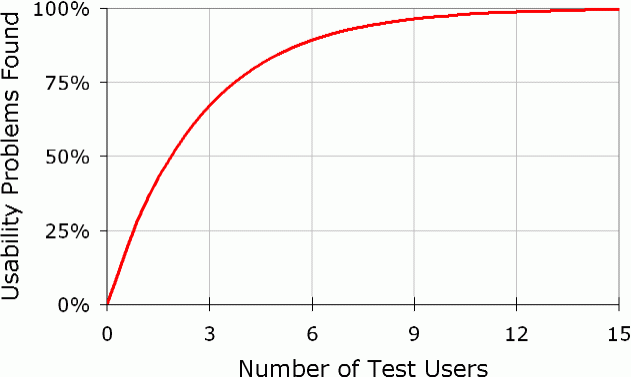
\includegraphics[width=1.0\textwidth]{number-of-test-users.png}
\caption{\label{fig:frog}User Tests}
\end{figure}

We usually met the users on their office since they have the material diagnostic with them and to observe the behaviour on their environment. We give them our machines to show the prototypes or just have an open interview to make some questions about the goals and the tasks to be concluded. It is important that each time we prepare a new user test session, we meet to define the learning goals, i.e. assumptions that need to be verified or might be proven wrong. For instance, when observing the clinic on their behaviour we understood the less usage of the keyboard against a very used mouse features.

\clearpage

\section{Learning Goals}

A test result is reliable only if it has been performed with the right kind of users. In our case, small number of profiles may interact with the user interface: Radiologists, Gynecologists, etc... So we make sure to target the right persona and just focus on that profile of clinicians. If we do not follow this rule and ask a tester to play a role, we will only get hypothetical answers to hypothetical problems.

A good preparation is essential to make the most out of the user tests. Testing just for the sake of testing is not enough, at best the researcher would give you a script with features list. Each time we prepare a new user test session, the researchers meet to define the learning goals, i.e. assumptions that need to be be verified or might be proven wrong. For instance, when we redesigned the user interface dedicated to a task, one assumption we had to test was that every essential information was easily accessible in the right menu against a right click option.

The learning goals are:

\ding{226} Understand how to annotate breast mass on our prototype;

\ding{226} Understand how to annotate breast calcification on our prototype;

\ding{226} Understand how to undo some annotation;

\ding{226} Understand how to redo some action on the prototype;

\ding{226} Understand how to erase some annotation on the prototype;

We neither pretend to have found the ultimate recipe for user testing, nor to have invented it. We merely absorbed and digested many good practices found elsewhere and tried to summarize it into our own process. What worked for our research project might not work “as is” for others, but we hope it will help us get started with user tests or maybe serve as an inspiration for future work about learning goals.

\clearpage

\section{Surveys vs Interviews (TODO: Re-write)}

One of the most important issues in the design of usable applications \cite{johnson2005user} is to learn about the people who will be using the application. This information is needed because different types of users require different types of interfaces \cite{nielsen1994usability}. Novice users, for example, will require frequent informative feedback as opposed to expert users who will require rapid response time and the availability of shortcuts \cite{shneiderman1987designing} and \cite{welch1998human}. A user analysis profiles the characteristics of the intended users of the system, such as age, education, skill level, cultural background, goals, computer literacy level, frequency of use, and familiarity with the domain. User capabilities can be determined through a survey/interview approach, direct interview, or direct observation \cite{strasberg1998moving}, \cite{hackos1997user} and \cite{shneiderman1987designing}. A major goal in the development of usable health care software should be to design a system that matches user’s capabilities.

Environmental analysis specifies the conditions in which systems are used. Several aspects of the physical environment are significant to the design of the interface. The place and conditions in which the system is used can be a deciding determinant for the type of interaction the user has with the system and the user’s progress with the system \cite{bouwhuis2000parts}. Examining environmental issues such as space, lighting, noise, availability of resources, danger, speed, power sources, and social and cultural issues are an integral part of the environmental analysis \cite{hackos1997user}.

The social environment of the users can impact the success or failure of a system. Social issues that need to be addressed as part of an environmental analysis are:

(1) Do the users share information and work together;

(2) Are resources readily available to assist the users \cite{hackos1997user}.

Cultural issues are significant to consider and not only relate to ethnicity, but also to socioeconomic status, professional status, and regional differences. These differences can affect working routines, interactions with others, values, and biases \cite{hackos1997user}. Taking the characteristics of the users and the environment into account addresses only two points of the triad of good human–computer interaction design. The users’ tasks must also be considered using a technique called task analysis. We must also consider the users’ tasks by using a technique called task analysis.

\section{Questions}

The following questions were made to the clinicians:

- Ask the question about having the BIRAD in each diagnosis image?

- Is it better on the High-Fi Prototype to have the right-click with all option, just the right menu with the options or both?

- Is it useful to have the colours annotation option?

\section{Tasks Analysis}

Task Analysis is the name given in this report to any process that identifies and examines the tasks that must be performed by users when they interact with systems. It is a fundamental approach which assists in achieving higher safety, productivity and availability standards.

The section describes the task analysis approach, and gathers together and comprehensively describes the application of some major task analysis techniques, organizing them into a practical scripts. The scripts are aimed at clinical practitioners such as Clinics, Radiologists, Doctors, etc., with or without previous task analysis experience, who have a need to establish task requirements or to carry out task assessments for one or more of the following topics:

\ding{226} Allocation of function (between human and machine);

\ding{226} Person specification;

\ding{226} Task and user interface design;

\ding{226} Human reliability assessment;

\ding{226} Performance checking;

\ding{226} Problem searching;

\clearpage

Guidance is provided on which techniques to use to achieve human-system performance goals (e.g. efficient and effective allocation of function) in the most cost-effective manner. Application of this section will therefore assist organizations in choosing and applying the most appropriate technique(s) to meet their particular needs. Examples from some of these topic areas of when and where Task Analysis could usefully be applied are the following:

\ding{226} Where it is necessary to provide assurance that task allocation and feasibility are appropriate?

\ding{226} When operational feedback raises concerns over a particular human-machine
interface?

\ding{226} When the requirements for productivity have changed?

\ding{226} Where personnel characteristics are different?

\ding{226} Where a significantly different technology is being used?

\ding{226} Where the same task has to be performed in a different environment?

\ding{226} How to detect false positives?

This section to Task Analysis shows how and when various task analysis techniques can be used to address the above issues, and also gives practical insights into the use of these techniques. Additionally, it assists in planning task analysis applications during the life cycle of a system, at any stage from early design onwards, to achieve cost-effective results. Finally, a number of real case studies demonstrate how task analysis has actually been used in practice, and the impact that task analysis has had in these clinical applications.

\clearpage

\section{The Script}

Before the users test, the research writes a script that will serve as a roadmap and guideline that can be shared with all research team who lead this project. It is a way to have consistent and comparable results.

This script consists in:

\ding{226} A reminder of the learning goals.

\ding{226} A check-list of the set-up elements that should be available for the test.

\ding{226} A clear and objective task: the job the clinician has to complete. It generally implies achieving smaller tasks related to the learning goals.

\ding{226} A few demographic questions to ask at the end.

On this research phase we will strict the interaction with the user as a beginning phase to record and obtain a new preliminary information about the user needs, goals and tasks. However we already tested some prototypes with Dra. Cristina Ribeiro da Fonseca and Dra. Clara Aleluia, it is still possible and valuable to restart the all process.

\clearpage

\section{The Meetings}

\subsection{SAMS Hospital}

The meeting was held at 5:00 pm on February 23, 2017 at SAMS Hospital in Lisbon. Its purpose was to draw some conclusions from important tasks, usability and even functionalities (eg ask if BIRAD will make sense for each image).

The conversation began with the doctor informing me that I had bought a new book on tomography and that this would help in the problem domain, as well as helping our Professor Daniel Sim\~{o}es Lopes in his research work. Here we can realize that in fact Doctor Cristina is motivated to help this and other scientific works. The book integrates mammography and ultrasound with tomosynthesis. Then there are mammograms and sonographies as examples where later both are compared with the own tomosintese, being this the first book that leaves on tomosintese.

The question was promptly asked about the functionality of BIRAD in all diganostic images, to which the author clearly said that it does not make any sense and that the solution will be to dispose of this functionality at the end of the diagnosis as a whole. This is because in case we are analyzing a craniocaudal we need to have a half-oblique to be able to classify the set of incidences.

After this first dialog we then proceed to the user tests, starting with the first High-Fi Prototype following the scripts described in the previous section. She was then asked by the doctor to pass the lapis over the breast making a circumferential loading from the right side of the mouse to demonstrate what actions the interface offers to manipulate the image. It was immediately warned that the interface was at a very primitive stage so that there is no disinterest about the prototype. We start then as if from zero the user tests to the interface. Initially the doctor had difficulty understanding the interaction mechanisms of the 2011 MacBook Air.

\clearpage

The first task was to make a note of the mass that was in the breast. The doctor did not understand at first how she began to scratch in the image the circumference derived from not being accustomed to tinkering with MacBooks and macOS system. You were instructed to press the MacBook mouse as an informational note to aid in learning while using your MacBook. Here the doctor understands how the menu options that appear when clicking on the right side appear. The first thing the doctor asked was the advantage of having multiple colors. And it began by trying to understand what each of the functions does, having arrived correctly at the solution and giving the right answers. In the beginning the doctor went to get a "Black Pen" but only later realized the need to have to load on the left side of the mouse to draw the lines. After that I had a failed attempt to use the "Paint" program as an example to try to exemplify the interaction, but later seeing the difficulties that the doctor was experiencing when using the macbook told him that to draw would have to keep pressing with the left side. Then the doctor understood the mechanics of the system and learned that pressing and dragging the finger will then draw the circle. However he did not realize that by default a selected color already comes and can start scratching right away. This way the first thing you did for the task was to load with the right side of the mouse and select the black color. Even so, I had to be the one to exemplify it. After this I can do it without any problem and had a very quick learning of how the interface works. The doctor's accuracy was not at all the best, but this is derived from never having used these hardware. Soon after was asked to do "Undo" so the doctor in seconds accomplish the task almost immediately. Then he was asked to do "Redo", "Erase" and "Text Annotation". In relation to the "Erase" functionality, the doctor was informed that the line manipulation symbol ("hand") will have to appear in order to activate the option to eliminate the line. This task was quickly acquired.

In relation to the general opinion of the doctor, she found the interface easy to learn and very intuitive. After this, it was asked if he prefers to have the functionality of the image manipulation options loaded with the right side of the mouse or if he prefers to have a sidebar with the same always visible. The answer was to have the sidebar in order to better show what options we have. This is because there are more clicks, it is more annoying for the user completely covering the overall image of the image on the diagnostic image, being nothing practical.

\clearpage

The doctor took the opportunity to ask why she had so many colors of "pen" and realized immediately that it was for the reason of having several lesions, such as, Multicentric, where we have several foci of the same quadrant; Multifocal, multiple outbreaks in more than one quadrant; And finally, Unifocal, a quadrant, an injury. The doctor has done an exaggeration of "pens" and advised to only use 3 "pens". It then suggests removing the black "pen".

Again the doctor argued the usability of the interface saying that it was quite fun to manipulate the image. Which shows motivation in doing so.
All this comes from having annotations with various colors which allows a variety of annotation in the images.

Finally the doctor asked that more features would be placed by what were explained the ones that were in the right menu and some more.

\subsection{S\~{a}o Jos\'{e} Hospital}

On February 24, 2017 (Friday) I went to the S\~{a}o Jos\'{e} in Lisbon at 09:50 for a meeting with Doctor Jo\~{a}o Louren\c{c}o at 10:00 in the morning as agreed by e-mail.

When I arrived at the Hospital, I encountered an organizational problem, because it was difficult for the information about my arrival to be properly communicated to the Doctor, and I had to send an SMS later to the doctor. In the answer to the SMS, the Doctor said to meet in the meeting room of Radiology so I immediately asked in the reception of the same area where this room was. They gave me the incomplete information so I had to ask another person in the hall. Arriving at the Doctor already with a delay of 15min due to all this, he asked me to sit down and had the remaining 45min to deal with a problem on the phone.

I took advantage of this waiting time by using it to understand the surrounding environment where the doctor works. In this case, there was a large room with a meeting table in the middle and against the wall there were 6 monitors radiological diagnosis. The material seemed good and in good conditions, unlike the Hospital's infrastructure. I remember the monitors being Philips.

\clearpage

At approximately 11:00, I then began to approach and get to know the doctor as a future user of our interface, as well as the future collaborator of the project. Dr. Jo\~{a}o Louren\c{c}o \cite{joaoLourenco} specializes in Radiology and currently works at both Hospital S\~{a}o Jos\'{e} and CUF Clinic in Bel\'{e}m and Hospital CUF in Torres Vedras. Essentially, and in an area of ​​interest as a user, it uses a lot of RIS software to obtain patient information and PACS, in this case the Philips eSight program, for the radiologic diagnosis. The features you use most are annotations written on the image and change the various views (windows) of the screen. It also uses the functionality of "Reformations" that will have to be later analyzed by us, the researchers.

In explaining the subject was somewhat reluctant to the fact that the project in its interpretation does not bring any sense of scientific innovation. So I explained that a new form of diagnosis would be implemented with a machine-readable approach to clinicians. It was mentioned in the possible existence of two types of software already on the market, Computer-Aided Detection (CADe) and Computer-Aided Diagnosis (CADx) \cite{computerAidedDiagnosis}. The former has an integrated implementation with machine learning so we have to keep this in mind in the future.

\clearpage

\section{Conclusions}

This report demonstrates, through a research work, an user interface for develop and design participatory user tests for health care interfaces that incorporates well-documented user-centered design principles.  The methods we employed in our user interface show the benefits toward system usefulness, information quality, and interface quality. Health care is an intense information gathering activity and has a very complex organizational structure. Understanding the users, the environment, and their tasks is just the beginning when designing software or redesigning interfaces. Incorporating user-centered design principles throughout the design life cycle has the promise to assist in providing quality health care systems.

\clearpage

\section{Acknowledgements}

This report will help our research project in cooperation between ISR \cite{isr} and INESC-ID \cite{inescid} both are associate institutes of Instituto Superior T\'{e}cnico \cite{ist}, Universidade de Lisboa \cite{ul}. Throughout this challenging journey we had the untiring and patient support from our family and friends.

We would like to give a special thanks to Doctor Clara Aleluia, Doctor Cristina Ribeiro da Fonseca and Doctor Jo\~{a}o Louren\c{c}o who have cooperated with us tirelessly, thus making a major contribution to the national research and development of innovation in Portuguese clinical Information Systems.

We also want to thanks Bruno Cardoso, Rodrigo Louren\c{c}o, Bruno Oliveira, Tom\'{a}s Pinho, L\'{i}dia Freitas, Bruno Dias, Jo\~{a}o Miranda, Prof. Dr. Jacinto Nascimento, Prof. Dr. Daniel Gon\c{c}alves, Ana Beatriz Alves, Francisco Silveira, Joana Teixeira, Daniel Da Costa, Filipe Fernandes, In\^{e}s Fran\c{c}a Martins, Lu\'{i}s Ribeiro Gomes and Ricardo Cruz for helping, supporting and reviewing our work.

\clearpage

\printbibliography

\end{document}
